\subsection{Memcached}
\label{sec:mcd}

\begin{figure*}
\centering
%\vspace*{-0.3cm}  
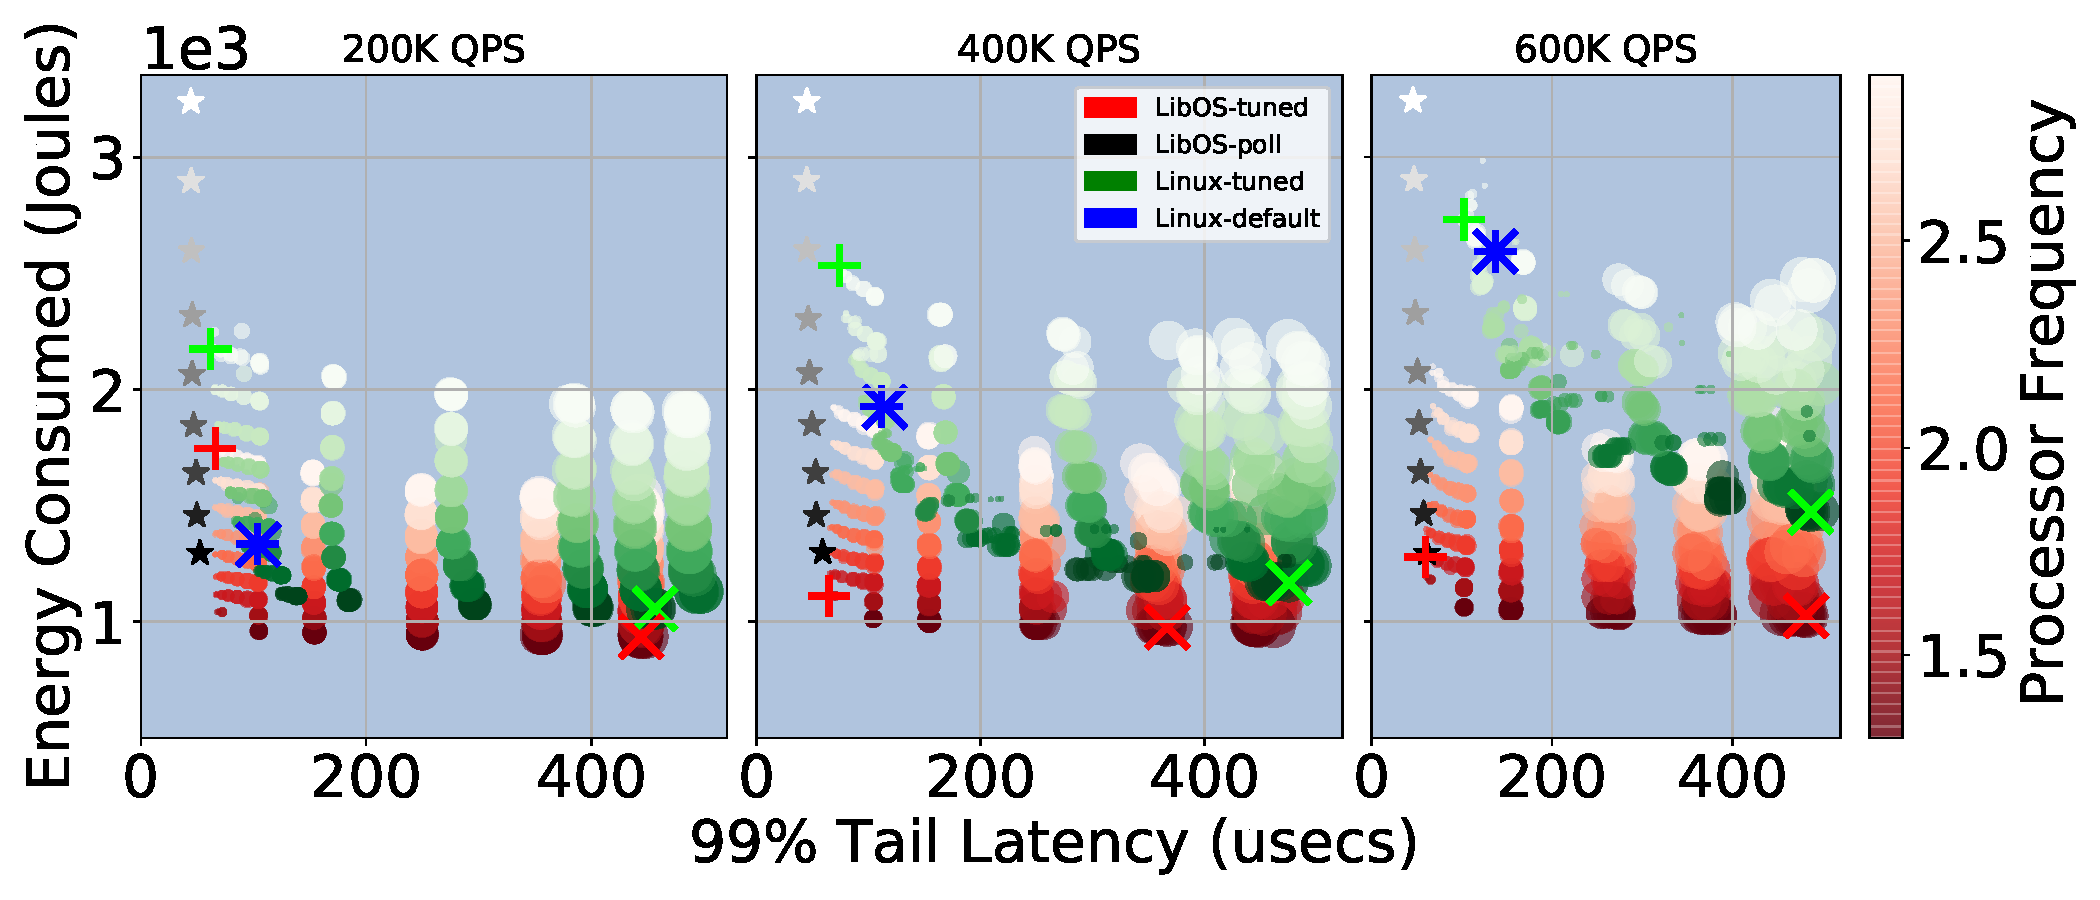
\includegraphics[width=1\textwidth]{figures/mcd_overview}
\caption[]
%{\small 
{Overview of memcached experiments across 200K, 400K, and 600K QPS. Each circle represents an experimental run of tuning ITR-delay and DVFS. The larger the size of a circle equates to larger ITR-delay value. The darkening of color gradient indicates slowing down processor frequency. The \textbf{x} indicate lowest energy consumption. The \textbf{+} indicate lowest tail latency.}
\label{fig:mcd_overview}
\end{figure*}

\begin{itemize}
    \item How we ran it, how many connections etc.
\end{itemize}

\subsubsection{Observable improvements when slowing down/speeding up}
\begin{itemize}
    \item See Figure~\ref{fig:mcd_overview}
    \item Linux-tuned over Linux-default: 1) energy savings when slowing down, 2) performance-energy trade-off when speeding up ITR
    \item LibOS-tuned: 1) energy savings when slowing down, 2) performance-energy trade-off when speeding up ITR
    \item LibOS-poll: 1) energy savings when slowing down
\end{itemize}

\begin{figure}
\centering
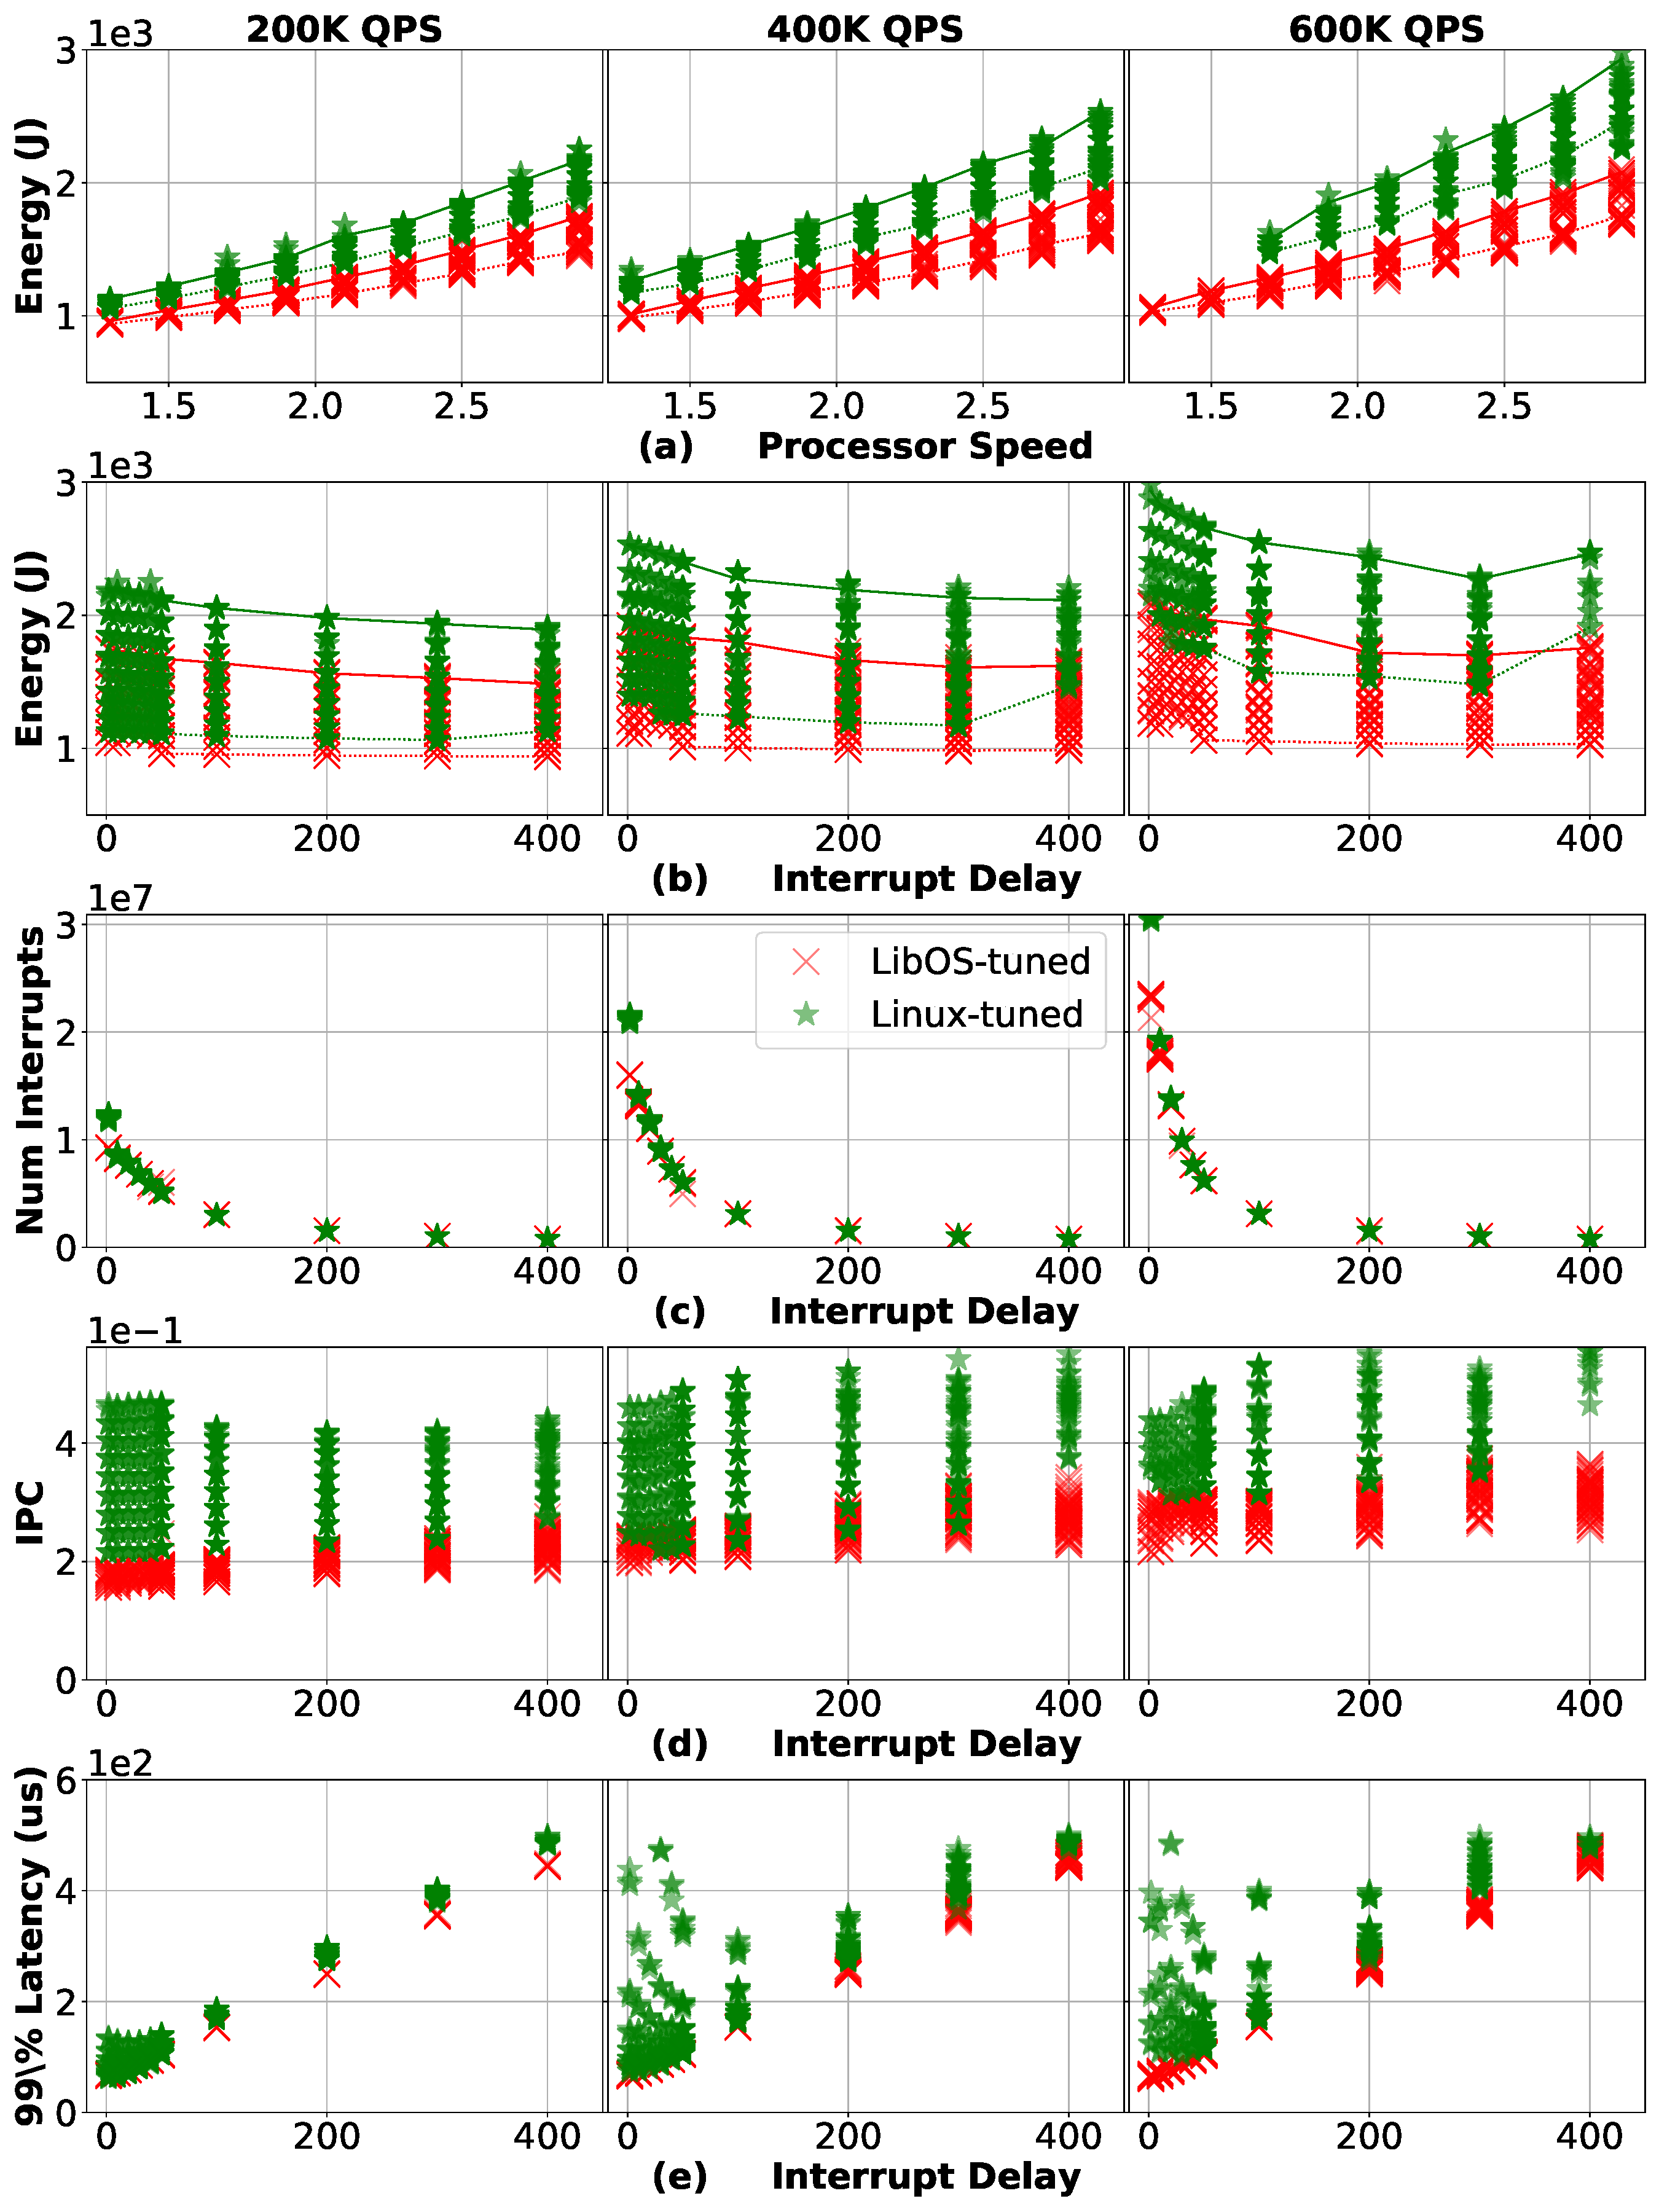
\includegraphics[width=0.5\textwidth]{figures/mcd_detail_1}
%\vspace*{-1.0cm}  
\caption[]{}
\label{fig:mcd_detail_1}
\end{figure}

\begin{figure}
  \centering
  \subfloat[a][a]{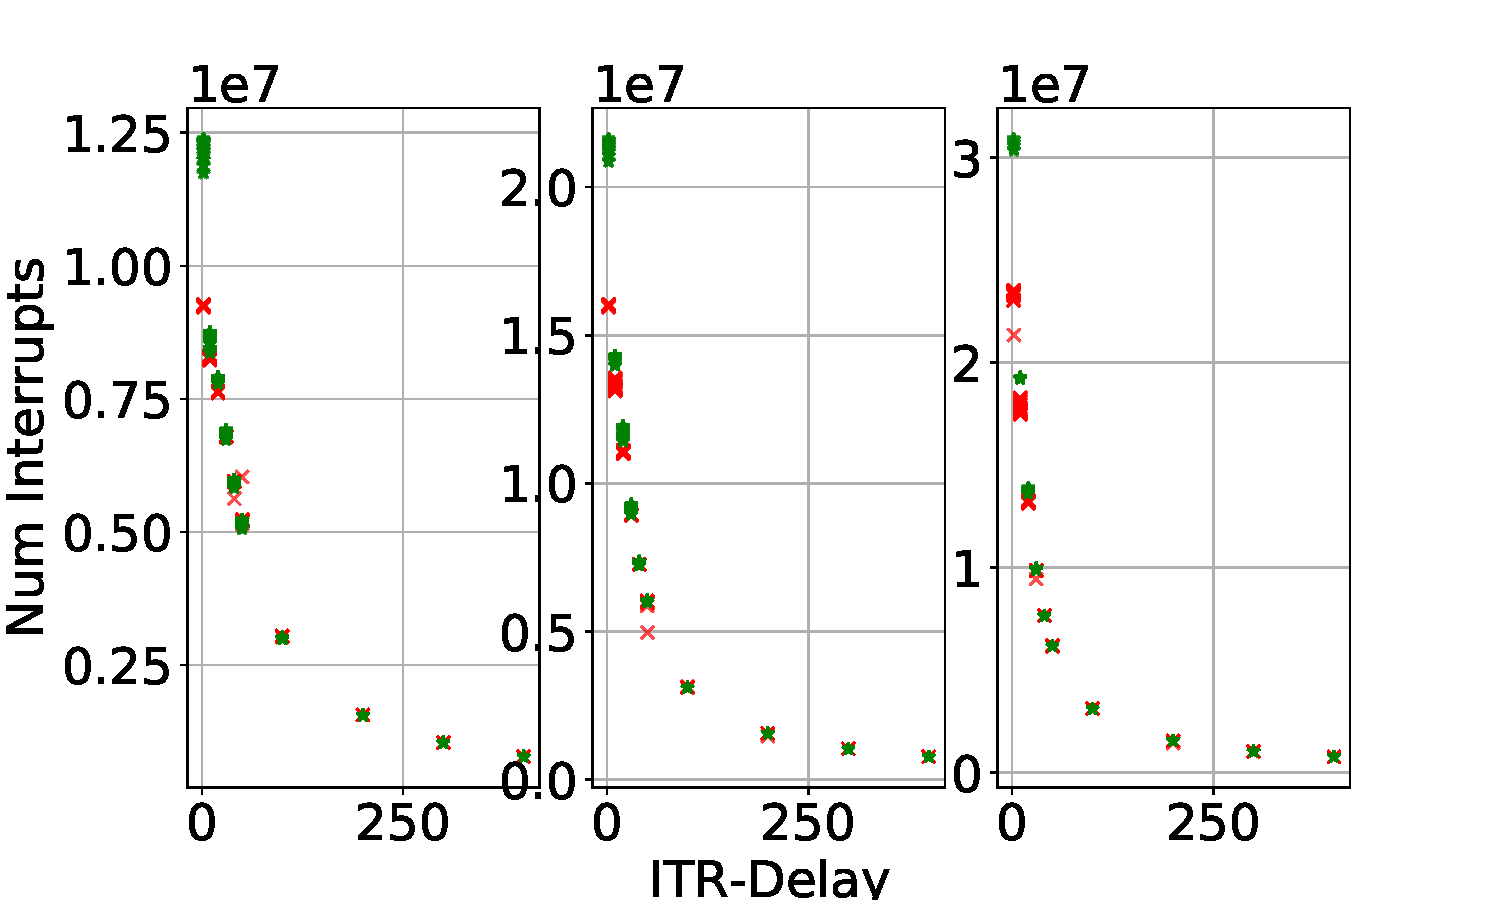
\includegraphics[width=0.45\textwidth]{sosp-21/figures/mcd_itr_num_interrupts.pdf}} \hfill
  \subfloat[b][b]{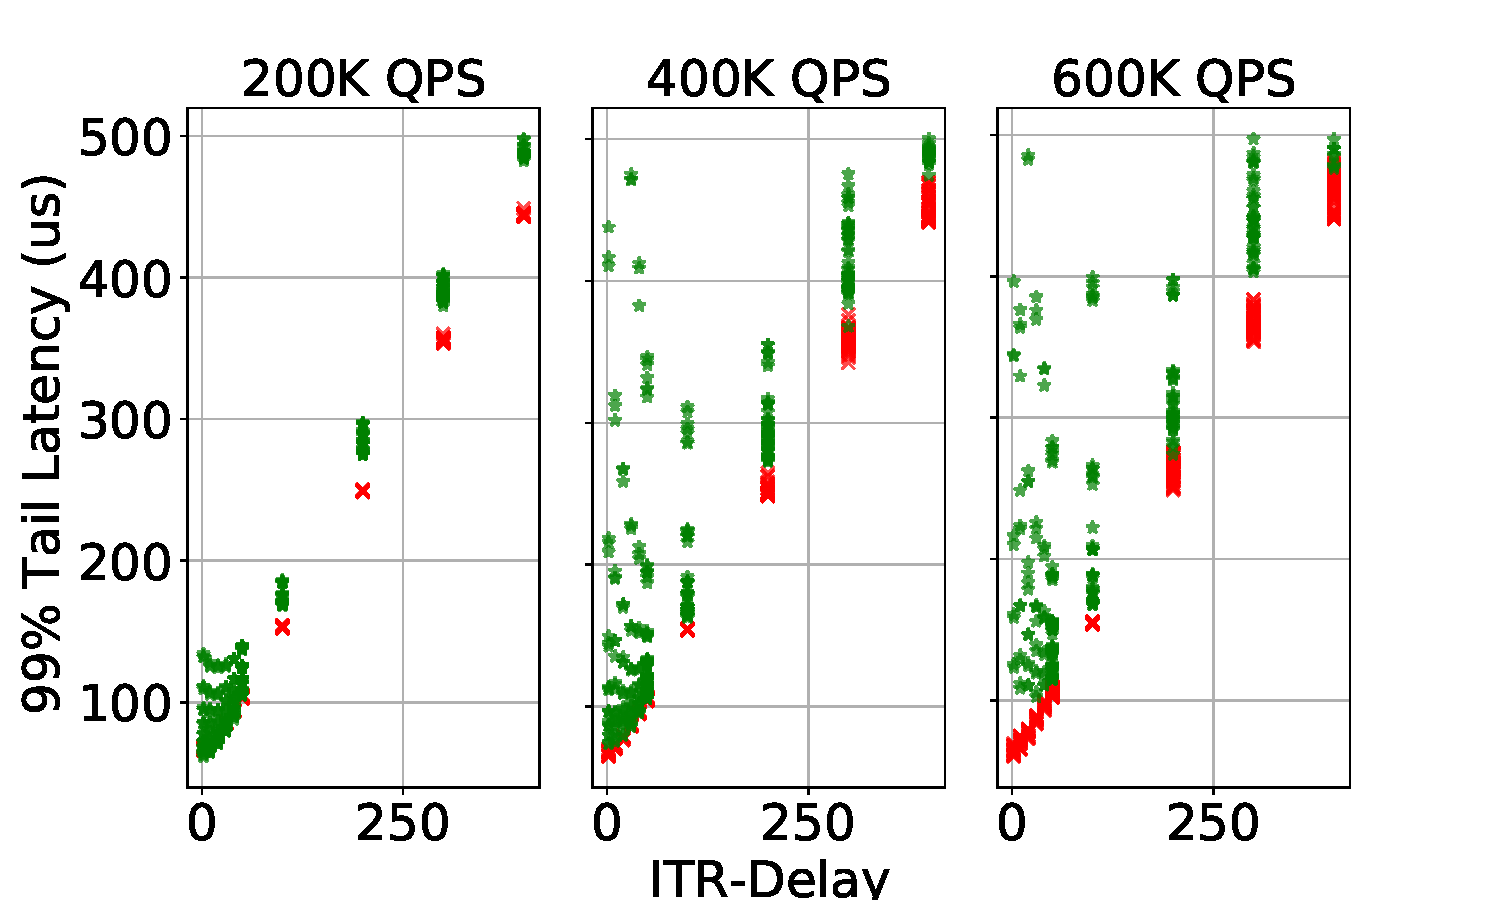
\includegraphics[width=0.45\textwidth]{sosp-21/figures/mcd_itr_read_99th.pdf}}
  %\caption{a + b} \label{fig:AB}
\end{figure}
    
% \begin{figure}
% \centering
% 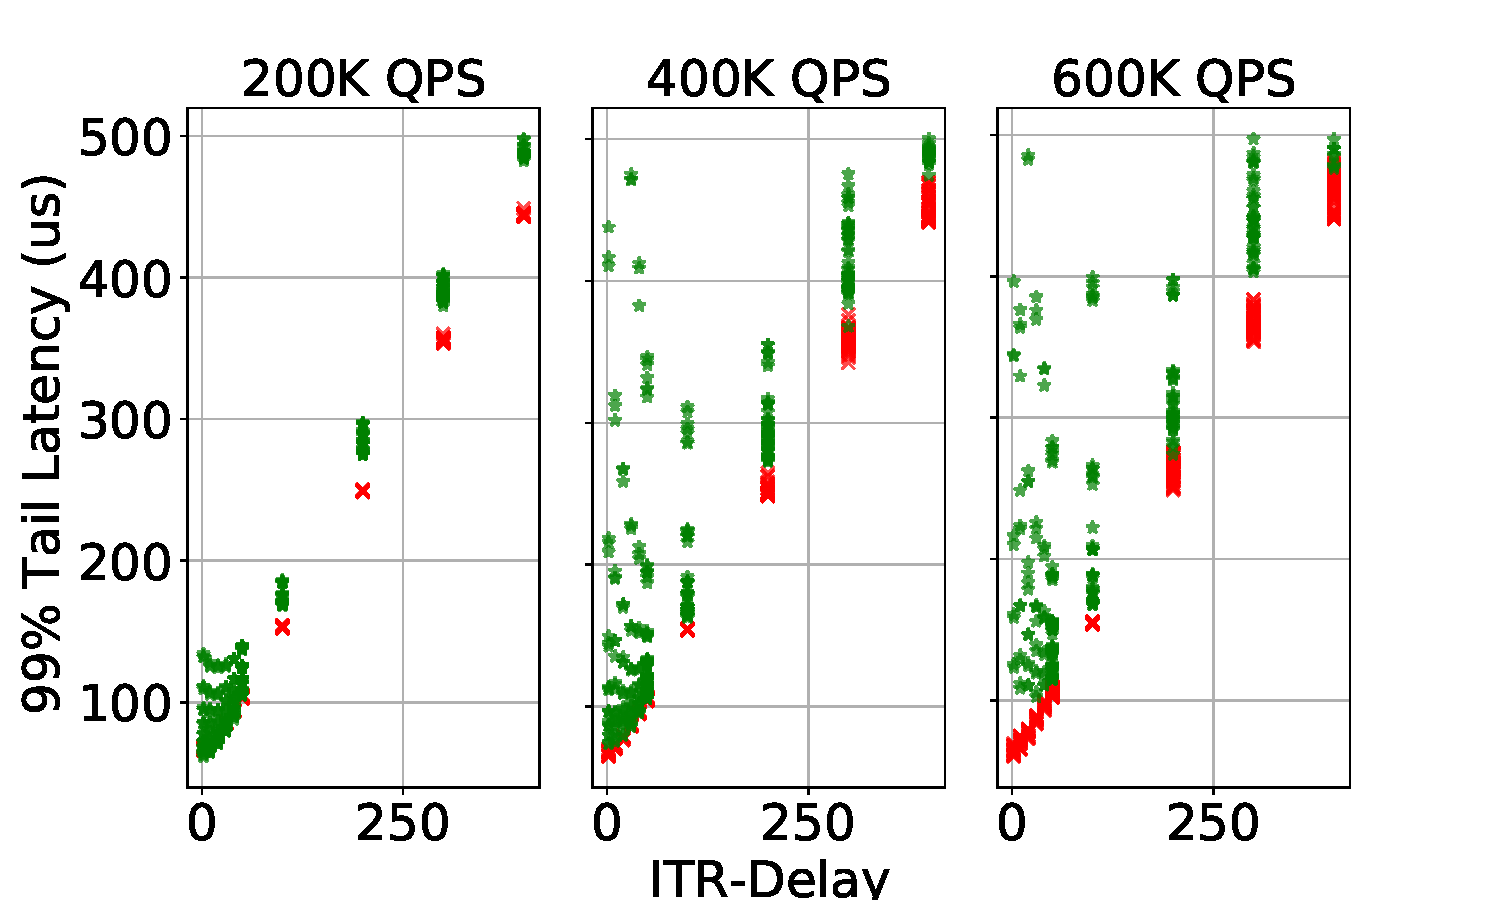
\includegraphics[width=0.5\textwidth]{sosp-21/figures/mcd_itr_read_99th.pdf}
% \vspace*{-0.7cm}  
% \caption[]{}
% \label{fig:mcd_itr_read99}
% \end{figure}

\begin{itemize}
    \item Figure~\ref{fig:mcd_detail_1}(a) shows energy fluctuations as function of DVFS. Bold lines indicate the mean energy consumption of the highest DVFS setting (fastest processor frequency). Dotted lines indicate mean energy consumption of lowest DVFS (slowest processor).
    \item Figure~\ref{fig:mcd_detail_1}(b)  shows energy fluctuations as function of ITR-Delay. Bold lines indicate mean energy consumption of highest ITR-Delay (fastest interrupt), dotted is slowest ITR-delay.
    \item 
\end{itemize}